\section{Auswertung}
\label{sec:Auswertung}
\subsection{Bestimmung der Filterkuve eines Selektivverstärkers}
Um die Filterkurve zu bestimmen, werden die gemessenen Ausgangsspannungen pro konstanter Eingangspannung $U_E = 100\si{\milli\volt}$ gegen die zugehörige Frequenz aufgetragen.
Die Kurve findet sich in Abbildung () und die Messwerte sind in Tabelle 1 aufgelistet. Für die Kurve werden nur die Werte um das Maximum aufgetragen, also von einer Frequenz von $\nu = 34 \si{\kilo\hertz}$ bis $\nu = 36 \si{\kilo\hertz}$.

\begin{table}[H]
  \centering
  \caption{Gemessene Ausgangsspannungen und zugehörige Frequenz.}
  \label{tab:Rechteckspannung}
  \begin{tabular}{c c}
    \toprule
    $\nu/$kHz & $U_A/$mV \\
    \midrule
20,0& 0,8 \\
21,0&	0,9\\
22,0&	1,0\\
23,0&	1,1\\
24,0&	1,2\\
25,0&	1,4\\
26,0&	1,5\\
27,0&	1,7\\
28,0&	2,1\\
29,0&	2,5\\
30,0&	3,1\\
31,0&	4,0\\
32,0&	5,3\\
33,0&	8,1\\
34,0&	15,4\\
34,1&	16,5\\
34,2&	18,4\\
34,3&	20,5\\
34,4&	23,5\\
34,5&	27,0\\
34,6&	31,0\\
34,7&	38,0\\
34,8&	47,0\\
34,9&	61,5\\
35,0&	82,0\\
35,1&	101,0\\
35,2&	94,5\\
35,3&	72,0\\
35,4&	54,0\\
35,5&	42,5\\
35,6&	34,5\\
35,7&	29,0\\
35,8&	25,6\\
35,9&	22,4\\
36,0&	19,9\\
37,0&	9,5\\
38,0&	6,2\\
39,0&	4,6\\
40,0&	3,7\\
      

   \bottomrule
  \end{tabular}
\end{table}

\begin{figure}[H]
  \centering
  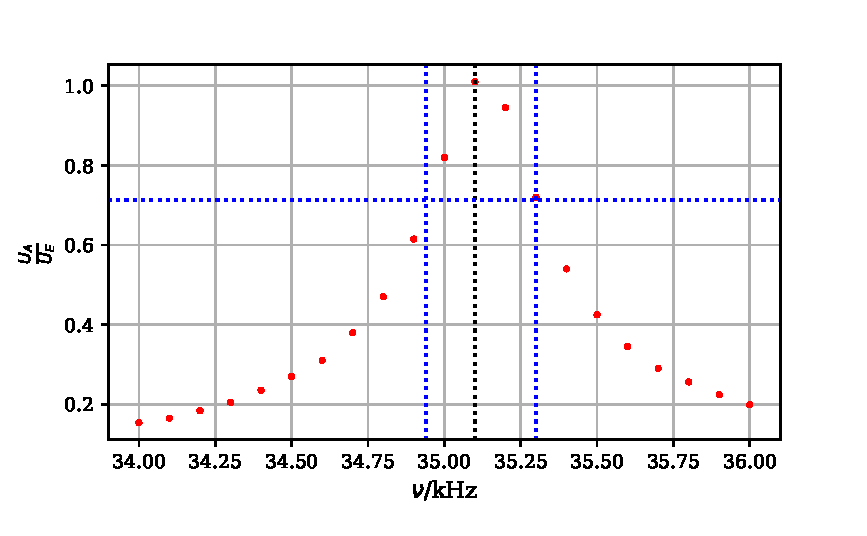
\includegraphics{plot1.pdf}
  \caption{Filterkurve eines Selektivverstärkers. }
  \label{fig:plot}
\end{figure}

Die maximale Spannung liegt bei $U_A = 101\si{\milli\volt}$ bei einer Frequenz von $\nu = 35,1\si{\kilo\hertz}$.
Die eingezeichneten vertikalen Linien geben die Maximale Frequenz und die Frequenzen an, bei denen die das Verhältnis der Spannungen auf einen Wert von $frac{1}{sqrt{2}}$ abgesunken ist.
Aus diesen drei Frequenzen lässt sich die Güte $Q$ der Kurve bestimmen
\begin{align*}
Q = \frac{\nu_0}{\nu_+ - \nu_-} = \frac{35,1}{35,3 - 34,94} = 97,5.
\end{align*}



\subsection{Berechnung der Suszeptibilität durch Messung}
In Tabelle 2 befinden sich die Messwerte zur Bestimmung der Suszeptibilität. Dabei sind $U_o$ und $R_o$ die gemessene Spannung bzw. der Widerstand ohne Probe, und $U_m$ und $R_m$ dementsprechend mit Probe.
$\Delta U$ und $\Delta R$ beschreiben die Differenz der beiden Spannungen und der Widerstände, denn diese Werte werden zur Suszeptibilitätsbestimmung gebraucht.
\begin{table}[H]
  \centering
  \caption{Messwerte zur Bestimmung der Suszeptibilitäten.}
  \label{tab:Widerstand}
  \begin{tabular}{c c c c c c c}
    \toprule
    Probe & $R_o / \symup{m\Omega}$   & $U_o / \symup{mV}\cdot 10^{-2}$  & $U_m / \symup{mV}\cdot 10^{-2}$ & $R_m / \symup{m\Omega}$ & $\Delta R / \symup{m\Omega}$ & $\Delta U / \symup{mV}\cdot 10^{-2}$  \\
    \midrule
    Dy & 3130 & 1,24 & 17,0 & 1600 & 1530 &15,76 \\
       & 3130 & 1,30 & 17,0 & 1600 & 1530 &15,70\\
       & 3165 & 1,31 & 17,4 & 1595 & 1570 &16,09\\
    Nd & 3130 & 1,28 & 1,50 & 3016 & 114 & 0,22\\
       & 3155 & 1,27 & 1,69 & 3016 & 139 & 0,42\\
       & 3140 & 1,26 & 1,50 & 3030 &110 & 0,24\\
    Pr & 3140 & 1,25 & 1,26 & 3100 &40 & 0,01\\
       & 3130 & 1,24 & 1,29 & 3075 &55 & 0,05\\
       & 3150 & 1,25 & 1,29 & 3095 &55 & 0,05\\
    Gd & 3140 & 1,25 & 8,80 & 2350 &790 &7,55\\
       & 3125 & 1,26 & 8,30 & 2370 &755 & 7,04\\
       & 3155 & 1,25 & 9,00 & 2375 &780 & 7,75\\


    \bottomrule
  \end{tabular}
\end{table}
\noindent In folgender Tabelle 3 sind die Mittelwerte der Differenz $\Delta U$ und $\Delta R$ aufgezählt.
Sie und ihre Fehler können mit den Formeln
\begin{align*}
x &= \frac{1}{3}\cdot \sum_{n=1}^{3} x_i\\
\Delta x &=\frac{1}{\sqrt{3}} \cdot \sqrt{\frac{1}{2} \sum_{n=1}^{3} (x_i - x)^2} 
\end{align*}
berechnet werden.
\begin{table}[H]
  \centering
  \caption{Mittelwerte der Messwerte zur Bestimmung der Suszeptibilitäten.}
  \label{tab:Widerstand}
  \begin{tabular}{c c c}
    \toprule
    Probe  &  $\Delta R / \symup{m\Omega}$ & $\Delta U / \symup{mV}\cdot 10^{-2}$  \\
    \midrule
    Dy & 1543,33 $\pm$ 18,86 & 15,85 $\pm$ 0,17 \\
    Nd & 121,0 $\pm$ 12,83 & 0,29 $\pm$ 0,09\\
    Pr & 50,0 $\pm$ 7,07 & 0,037 $\pm$ 0,019 \\
    Gd & 775,0 $\pm$ 14,72 & 7,45 $\pm$ 0,299\\
    \bottomrule
  \end{tabular}
\end{table}

Die Abmessungen der Proben, also die Masse $m$, die Dichte $\rho$ und die Länge $L$, sind in Tabelle 4 aufgeführt. Dabei ist allerdings zu beachten, dass die Dichte für C6O12Pr2 nicht gefunden wurde, und deshalb die Dichte für Pr genommen wird.
\begin{table}[H]
  \centering
  \caption{Abmessungen der Proben.}
  \label{tab:Dy}
  \begin{tabular}{c c c c}
    \toprule
    Probe & $m/ \symup{g}$ & $\rho / \symup{\frac{g}{cm^3}}$   & $L / \symup{cm}$  \\
    \midrule
    Dy & 14,38 & 7,8 & 13,5\\
    Nd & 9,09 & 7,24 & 13,5\\
    Pr & 7,87 & 6,773 & 13,5 \\
    Gd & 14,08 & 7,40 & 13,5\\
    \bottomrule
  \end{tabular}
\end{table}
%http://www.periodensystem.info/elemente/praseodym/

\noindent Weitere Größen, die bekannt sein müssen, sind folgende:

\noindent Die Speisespannung beträgt $U_S = 0,71\si{\volt}$,

\noindent die Windungszahl der Spule beträgt $n = 250$,

\noindent der Widerstand der Spule beträgt $R = 0,7 \: \symup{\Omega}$,

\noindent und der Querschnitt der Spule beträgt  $F = 86,6 \: \symup{mm^2}$.

\noindent Außerdem lautet der Widerstand $R_3 = 998 \Omega$.

\subsection{Berechnung der Suszeptibilität für Dyprosium}
Mit Gleichung () kann der Querschnitt der Probe ausgerechnet werden
\begin{align*}
Q_{real} = \frac{m}{L \cdot \rho}
\end{align*}
\begin{align*}
Q_{Dy} = 13,66 \si{\milli\meter}^2
\end{align*}
Die Suszeptibilität bestimmt sich durch Gleichungen () und () auf zwei Weisen
\begin{align*}
\chi_{Dy_U} = 0,0566 \pm 0,0006 \\
\chi_{Dy_R} = 0,1961 \pm 0,0024 .
\end{align*}

\subsection{Berechnung der Suszeptibilität für Neodym}
Der reale Querchnitt berechnet sich zu
\begin{align*}
Q_{Ny} = 9,3 \si{\milli\meter}^2
\end{align*}
Die Suszeptibilität bestimmt sich durch Gleichungen () und () auf zwei Weisen
\begin{align*}
\chi_{Ny_U} = 0,0015 \pm 0,0005 \\
\chi_{Ny_R} = 0,0226 \pm 0,0024 .
\end{align*}

\subsection{Berechnung der Suszeptibilität für Praseodym}
Der reale Querchnitt berechnet sich zu
\begin{align*}
Q_{Pr} = 8,61 \si{\milli\meter}^2
\end{align*}
Die Suszeptibilität bestimmt sich durch Gleichungen () und () auf zwei Weisen
\begin{align*}
\chi_{Pr_U} = 0,0002 \pm 0,0001 \\
\chi_{Pr_R} = 0,0101 \pm 0,0014 .
\end{align*}

\subsection{Berechnung der Suszeptibilität für Gadolinium}
Der reale Querchnitt berechnet sich zu
\begin{align*}
Q_{Gd} = 14,09 \si{\milli\meter}^2
\end{align*}
Die Suszeptibilität bestimmt sich durch Gleichungen () und () auf zwei Weisen
\begin{align*}
\chi_{Gd_U} = 0,0258 \pm 0,0010 \\
\chi_{Gd_R} = 0,0954 \pm 0,0018 .
\end{align*}


\subsection{Theoretische Berechnung der Suszeptibilität}
Theoretisch berechnet werden kann die Suszeptibilität mit Gleichung (). Dazu benötigt man den Land$\acute{\text{e}}$-Faktor $g_J$. Den Spin, Bahndrehimpuls und den Gesamtdrehimpuls berechnet man aus den Hundschen Regeln.
Das Element Dy hat neun 4f-Elektronen, Gd hat sieben, und Nd hat drei. Als Beispiel zur Berechnung der Größen wird Dyprosium verwendet.
In die 4f-Schale passen 14 Elektronen. Das f steht für den maximalen Drehimpuls $l = 3$. 
Die Orbitale werden laut den Hundschen Regeln immer erst einzeln besetzt. Deshalb sind nur zwei Orbitale vollständig gefüllt. 5 Orbitale haben nur Elektronen mit Spin $\frac{1}{2}$, und diese addieren sich dann laut der ersten Regel zu $S= 2,5$.
Da die Drehimpulse maximal sein sollen, hat das erste Orbital $l=3$, das zweite $l_2$ und so weiter bis $l=-3$.
Da aber nur die ersten beiden vollständig besetzt sind, zählen nur diese und der Drehimpuls ergibt sich zu $L=3+2=5$.
Der Gesamtspin $J$ ist die Addition von L und S, also $J=2,5+5=7,5$, da die Schale mehr als die Hälfte gefüllt ist.
In einer Tabelle sind alle Werte für alle Elemente notiert, und dazu auch der sich aus Gleichung () ergebende Land$\acute{\text{e}}$-Faktor.
\begin{table}[H]
  \centering
  \caption{Gesamtspin, Bahndrehimpuls, Gesamtdrehimpuls und Land$\acute{\text{e}}$-Faktor der Proben}
  \label{tab:Dy}
  \begin{tabular}{c c c c c}
    \toprule
    Probe & $L$ & $S$ & $J$  & $g_J$  \\
    \midrule
    Dy & 5 & 2,5 & 7,5 & 1,33\\
    Pr & 5 & 1 & 4 & 0,8 \\
    Nd & 6 & 1,5 & 4,5 & 0,73\\
    Gd & 0 & 3,5 & 3,5 & 2,00\\
    \bottomrule
  \end{tabular}
\end{table}

Die Werte für $N$ lauten nach der Formel $N=\frac{2 \rho N_{\symup{A}}}{M}$
\begin{align*}
  N_{Dy} = 2,52 \cdot 10^{28} \si{\per\meter^3}\\
  N_{Pr} = 1,49 \cdot 10^{28} \si{\per\meter^3}\\
  N_{Nd} = 2,59 \cdot 10^{28} \si{\per\meter^3}\\
  N_{Gd} = 2,46 \cdot 10^{28} \si{\per\meter^3}\\
 \end{align*}
wobei $N_A$ die Avogadrokonstante und $M$ die molare Masse ist.
Diese molaren Massen sind laut .... für die Elemente
\begin{align*}
  M_{Dy} = 373,00 \frac{g}{mol} \\
  M_{Pr} = 545,87 \frac{g}{mol} \\
  M_{Nd} = 336,48 \frac{g}{mol} \\
  M_{Gd} = 362,49 \frac{g}{mol} \\
\end{align*}
Es wird eine Raumtemperatur von $295,15 \si{\kelvin}$ angenommen.
Die Suszeptibilitäten ergeben sich also zu
\begin{align*}
\chi_{Dy_T} = 0,0251 \\
\chi_{Pr_T} = 0,00169 \\
\chi_{Nd_T} = 0,00302 \\
\chi_{Gd_T} = 0,0137 \\
\end{align*}
